%%%%%%%%%%%%%%%%%%%%%%%%%%%%%%%%%%%%%%%%%%
% Creator : Amir Adib SAbbag
% Github: github.com/Amir1453
%%%%%%%%%%%%%%%%%%%%%%%%%%%%%%%%%%%%%%%%%%
% Star if you like it please!
%
% If you want to add a picture add it to ./images
% 
% You must create the first page in a different place (photoshop, word etc.) and then you can combine the two.
%--------------------------------------
% 
% If you are going to use babel with Turkish then you have to use
%
%\shorthandoff{=}
%\begin{figure}[H]
%    \centering
%    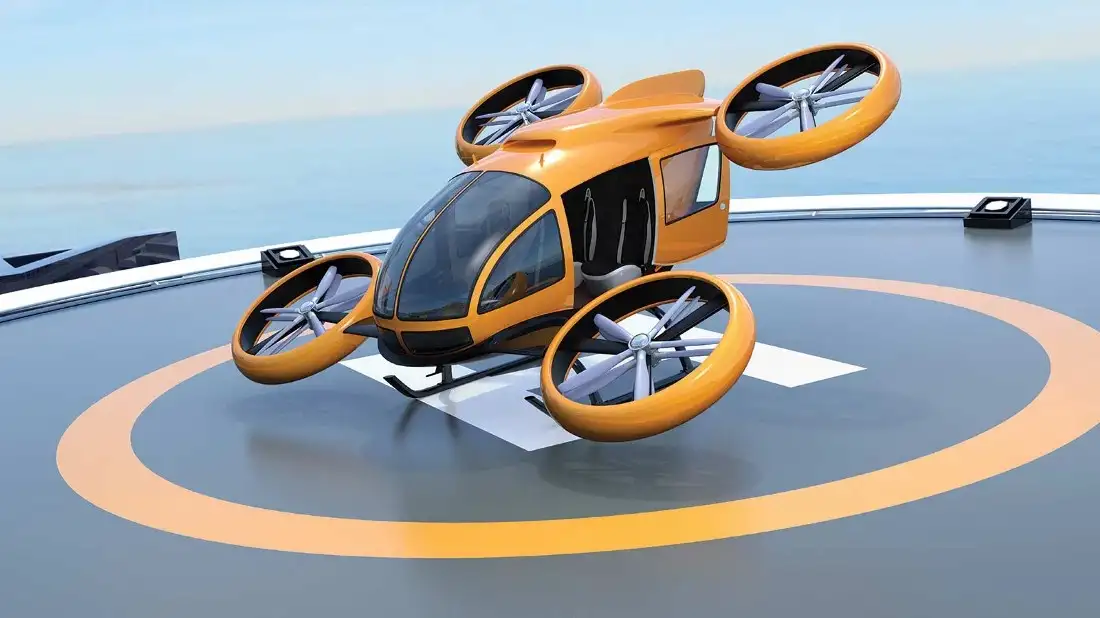
\includegraphics[scale=0.40]{images/flyingcar.png}
%    \caption{Caption}
%    \label{fig:my_label}
%\end{figure}
%\shorthandon{=}
%
% When adding images because there is a bug with the Turkish version of babel.
% IF you are going to use the English version, you dont have to use \shorthandoff{=} and \shorthandon{=}
%-------------------------------------------
%
% To add a reference use \cite{}
% You can add your references to bibliography.bib in the bibtex format.
% For more information please check out
% https://www.overleaf.com/learn/latex/Bibliography_management_with_bibtex
%-----------------------------------------
% You can add categories with
% Section, subsection, subsubsection paragraph 
% \tableofcontents will automatically create a table of contents for you.
%-----------------------------------------
% You can make any changes you wish, it is up to you.
% If your particular project has different constraints you can change it to fit to them.
% If you have any questions open an issue!
%-------------------------------------------




%establishing document class with 12pt
\documentclass[12pt]{article}



%\usepackage[turkish]{babel}%Turkish
\usepackage[english]{babel} %English
\usepackage[utf8]{inputenc} %utf8
%\usepackage[T1]{fontenc} %Turkish spelling

%Packages used for the background image and images

\usepackage{xcolor}
\usepackage{graphicx}
\graphicspath{./images}
\usepackage{float}
\usepackage{eso-pic}
\usepackage[export]{adjustbox}

%Package used for making hyperlinks
\usepackage[hidelinks]{hyperref}

%Times New Roman Font
\usepackage{times}

% for reference urls to work.
\usepackage{url}

%Package for bibliography
\usepackage[sorting=none,backend=bibtex]{biblatex}
\addbibresource{bibliography.bib}

%Adding TEKNOFEST watermark.
\newcommand\BackgroundPicture{
   \put(0,0){
     \parbox[b][\paperheight]{\paperwidth}{
       \vfill
       \centering
\includegraphics[width=0.7\paperwidth,height=0.7\paperheight,keepaspectratio]{background.png}
       \vfill
     }}}
\AddToShipoutPicture{\BackgroundPicture}



% To make create the file within TEKNOFEST constraints
% Page numbering on top right and author name in middle below
% IF YOUR PARTICULAR PROJECT REQUIRES SOMETHING ELSE CHANGE IT HERE!
\usepackage{fancyhdr}
\pagestyle{fancy}
\renewcommand{\headrulewidth}{0pt}
\fancyhf{}
\fancyhead[R]{\thepage}
%enter your team name here
\fancyfoot[C]{TEAM NAME}



%Begin the document
\begin{document}

\begin{center}
    \Huge BLANK PAGE    
\end{center}

% Leaves the first page blank so that you can add your own cover page.
\newpage

%Creating a table of contents
\tableofcontents

%leaves a blank page after creating the index
\newpage



% General section
% Dont forget you can create your sections and subsections!
% The sections provided below are just examples.
\section{Senaryo ve Hava Trafik Yöntemi}

% YOU CAN ADD TEXT HERE!

\subsection{Genel Trafik Modeli}
% YOU CAN ADD TEXT HERE!

\subsection{Hava Araçlarının Hareket Kuralları}
% YOU CAN ADD TEXT HERE!
\subsubsection{Araçların kurallara uyabilmesi için gereken özellikler}
% YOU CAN ADD TEXT HERE!
\subsubsection{Kullanıcıların Yükümlülükleri}
% YOU CAN ADD TEXT HERE!
\subsubsection{Kurallara uyulmaması durumunda yaptırımlar}
% YOU CAN ADD TEXT HERE!
\subsubsection{Hava araçlarının tam otonom olma süreci}
% YOU CAN ADD TEXT HERE!

\subsection{Hava Araçlarında Komünikasyon}

\subsubsection{Araçlar arası komünikasyon}
% YOU CAN ADD TEXT HERE!
\subsubsection{Araçlar ve merkez arası komünikasyon}
% YOU CAN ADD TEXT HERE!
\subsubsection{Araçlar ve kalkış iniş noktaları arası komünikasyon}
% YOU CAN ADD TEXT HERE!

\subsection{Araca Biniş ve İniş}

\subsubsection{Merkezi duraklar}
% YOU CAN ADD TEXT HERE!
\subsubsection{Bireysel kullanım}
% YOU CAN ADD TEXT HERE!

\subsection{Rota Planlama}

\subsubsection{Varış noktası seçimi}
% YOU CAN ADD TEXT HERE!
\subsubsection{Seyahat sırasında daha optimal rota tespiti}
% YOU CAN ADD TEXT HERE!
\subsubsection{Kullanıcı tarafından varış noktasının değiştirilmesi}
% YOU CAN ADD TEXT HERE!
\subsubsection{Şehir içi ve dışı rotalar}
% YOU CAN ADD TEXT HERE!

\subsection{İdeal Olmayan Durumlara Karşı Tepki}
% YOU CAN ADD TEXT HERE!
\subsubsection{Değişken hava durumu}
% YOU CAN ADD TEXT HERE!
\subsubsection{Beklenmedik trafik yoğunluğu}
% YOU CAN ADD TEXT HERE!
\subsubsection{Acil durumlar}
% YOU CAN ADD TEXT HERE!

\subsection{Yakıt/Batarya}
% YOU CAN ADD TEXT HERE!
\subsubsection{Batarya/yakıt kapasitesinin yönetimi}
% YOU CAN ADD TEXT HERE!
\subsubsection{Şarj/dolumun hangi aralıklarla yapılacağı}
% YOU CAN ADD TEXT HERE!
\subsubsection{Şarj/dolumun nerede yapılacağı}
% YOU CAN ADD TEXT HERE!

% Adding a new page after all the text.

\newpage

% If there is anything that you did not cite but want to add to the references add it to \nocite{}
%\nocite{citekey,citekey2}
% Prints all the references.
\printbibliography
    
\end{document}
